\documentclass[10pt,a4paper]{article}
\usepackage[paper=a4paper, hmargin=1.5cm, bottom=1.5cm, top=3cm]{geometry}

\usepackage[utf8x]{inputenc}
\usepackage[spanish]{babel}

\usepackage{mathtools}
\usepackage{amsmath}
\usepackage{amsfonts}
\usepackage{amssymb}

\usepackage{xcolor}
\usepackage{listingsutf8}
\usepackage{booktabs}
\usepackage{hyperref}
\usepackage{multirow}

\usepackage{caption}
\usepackage{subcaption}

\usepackage{algorithm}
\usepackage[noend]{algpseudocode}

\usepackage{graphicx}
\usepackage{tikz}
\usepackage{relsize}
\usepackage{epstopdf}

\usepackage{chessboard}
\storechessboardstyle{6x6}{maxfield=h8}

\DeclarePairedDelimiter{\ceil}{\lceil}{\rceil}

%\let\NombreFuncion=\textsc
%\let\TipoVariable=\texttt

%\newcommand{\TipoFuncion}[3]{%
  %\NombreFuncion{#1}(#2) \ifx#3\empty\else $\to$ \res\,: \TipoVariable{#3}\fi%
%}

% set the default code style
\lstset{
    frame=tb, % draw a frame at the top and bottom of the code block
    tabsize=4, % tab space width
    showstringspaces=false, % don't mark spaces in strings
    numbers=left, % display line numbers on the left
    commentstyle=\color{green}, % comment color
    keywordstyle=\color{blue}, % keyword color
    stringstyle=\color{red} % string color
}

% mathy stuff
\newtheorem{theorem}{Theorem}[section]
\newtheorem{lemma}[theorem]{Lemma}
\newtheorem{proposition}[theorem]{Proposición}
\newtheorem{corollary}[theorem]{Corollary}

\newenvironment{proof}[1][Demostración]{\begin{trivlist}
\item[\hskip \labelsep {\bfseries #1}]}{\end{trivlist}}
\newenvironment{definition}[1][Definición]{\begin{trivlist}
\item[\hskip \labelsep {\bfseries #1}]}{\end{trivlist}}
\newenvironment{example}[1][Example]{\begin{trivlist}
\item[\hskip \labelsep {\bfseries #1}]}{\end{trivlist}}
\newenvironment{remark}[1][Remark]{\begin{trivlist}
\item[\hskip \labelsep {\bfseries #1}]}{\end{trivlist}}

\newcommand{\qed}{\nobreak \ifvmode \relax \else
      \ifdim\lastskip<1.5em \hskip-\lastskip
      \hskip1.5em plus0em minus0.5em \fi \nobreak
      \vrule height0.75em width0.5em depth0.25em\fi}

\title{Métodos Numéricos \\ TP1}

\newcommand{\order}[1]{$\mathcal{O}(#1)$}

\begin{document}

%% cover page

\maketitle

\bigskip

\begin{table}[h]
\centering
\begin{tabular}{|l l l|}
\hline
Integrante       & \multicolumn{1}{c}{LU}     & Correo electrónico        \\ \hline
Martin Baigorria & \multicolumn{1}{c}{575/14} & martinbaigorria@gmail.com \\ 
Federico Beuter & 827/13                      & federicobeuter@gmail.com \\
Mauro Cherubini & 835/13                      & cheru.mf@gmail.com \\ 
Rodrigo Kapobel & 695/12                      & rok\_35@live.com.ar \\  \hline
\end{tabular}
\end{table}

\begin{center}
\textbf{Reservado para la cátedra}
\end{center}
\begin{table}[h]
\centering
\begin{tabular}{|l|l|l|}
\hline
Instancia       & Docente & Nota \\ \hline
Primera entrega &         &      \\ \hline
Segunda entrega &         &      \\ \hline
\end{tabular}
\end{table}

\vfill
\textbf{Resumen:}
El siguiente trabajo practico tiene como objetivo implementar, utilizar y evaluar el método de eliminación gausiana y la factorización LU para resolver un problema que involucra la propagación del calor en la pared de un horno descripta con un laplaciano. Para ello se discretizara esta ecuación diferencial y luego se planteara un sistema matricial de la forma $Ax = b$ para calcular la temperatura en los diferentes puntos de la discretizacion en la pared del horno.
Se analizaran diferentes escenarios en las condiciones del problema para evaluar en que escenarios una factorización supera a la otra. Se evaluaran algunas cuestiones relacionadas con el problema en sí, como por ejemplo la presición de un algoritmo de búsqueda de isotermas en la pared del horno y la velocidad de convergencia a la isoterma teórica.
Finalmente concluimos que la factorización LU supera ampliamente a la eliminación gausiana en cuanto a complejidad temporal en escenarios donde cambia el vector $b$ de forma recurrente. A su vez, notamos que la presición del algoritmo de búsqueda de isotermas no es estrictamente decreciente en función de la discretización, aunque por supuesto mejora a medida que aumenta en múltiplos de 2.

\textbf{Keywords:} Gaussian Elimination, LU Factorization.

\newpage
\tableofcontents
\newpage

% end cover page

\section{Introducción}

Existe una gran variedad de problemas que pueden ser modelados por medio de sistemas de equaciones lineales. Estas ecuaciones pueden ser expresadas mediante un sistema matricial que se puede escribir de la forma $Ax = b$ donde $A \in \mathbb{R}^{n \times n}$ y $x,b \in \mathbb{R}^{n \times 1}$. Una vez representado, se debe buscar alguna forma de resolver el sistema, es decir, buscar el vector $x$. Existen numerosas maneras de resolver este problema, entre ellas tenemos por ejemplo el clásico algoritmo de eliminación gausiana y la factorización LU.

El objetivo de este trabajo practico es modelar y resolver el problema de la difusión del calor en la pared de un horno circular. A priori, lo que sabemos es que el calor se propaga siguiendo la ecuación diferencial dada por el laplaciano en función del angulo y la distancia desde el centro del horno. Aunque esta ecuación diferencial tiene una solución analítica, el trabajo practico apunta a que modelemos este problema discretizando el dominio en coordenadas polares y planteando el sistema de ecuaciones dado por el laplaciano de forma matricial. De esta forma podemos encontrar una aproximación de la temperatura en cada punto de la discretización.

El horno tiene una característica muy particular.  La isoterma 500$^{\circ}$C debe encontrarse dentro de la pared del mismo para no comprometer su integridad estructural. Por esta razón, uno de los objetivos una vez que hemos calculado la temperatura aproximada en diferentes puntos de la discretización es encontrar de alguna forma esta isoterma y ver si el horno es estable dependiendo de la temperatura interna y externa del mismo. Para ello propondremos diferentes algoritmos que dada la discretización aproximen la ubicación de la misma. Estas problemáticas se pueden ver claramente en las siguientes figuras:

\begin{figure}[h]
  \centering
  \begin{minipage}[b]{0.35\textwidth}
    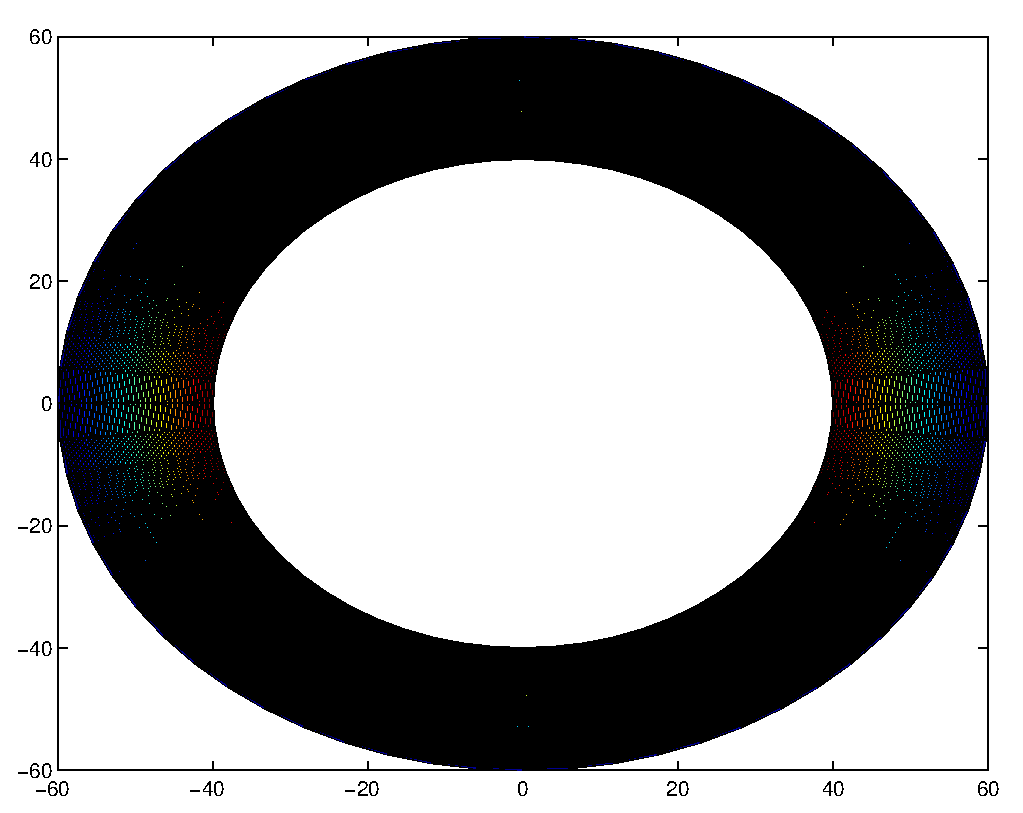
\includegraphics[width=\textwidth]{graficos/isotermaIdeal_heat.eps}
    \caption{Heat map.}
  \end{minipage}
  \hspace{1cm}
  \begin{minipage}[b]{0.30\textwidth}
    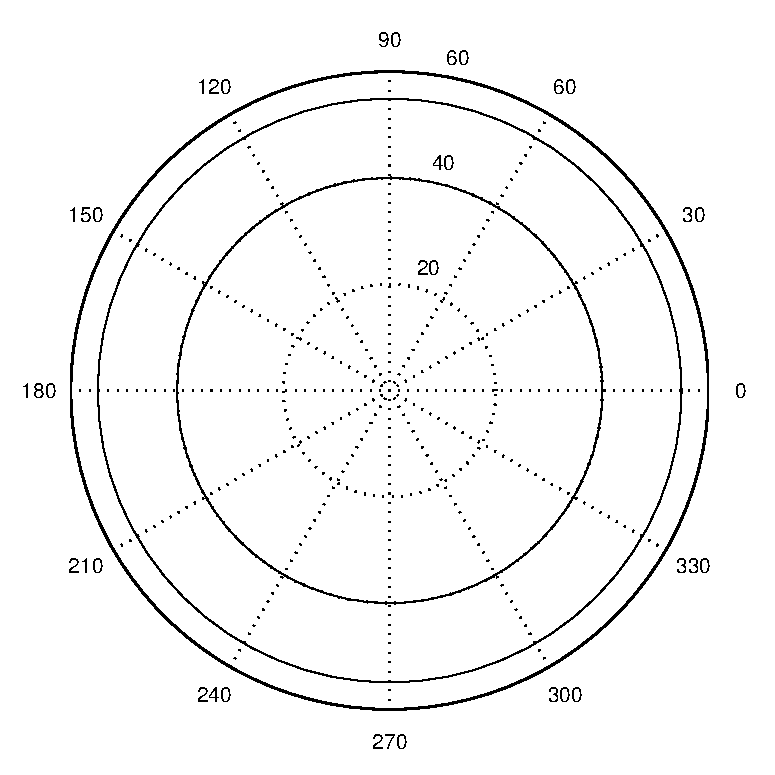
\includegraphics[width=\textwidth]{graficos/isotermaIdeal.eps}
    \caption{Isoterma.}
  \end{minipage}
\end{figure}

En el heat map se puede ver como la temperatura representada con colores va bajando a medida que uno se aleja de la pared interna del horno. A su vez, en el gráfico de la isoterma podemos ver la pared interna del horno y la isoterma 500$^{\circ}$C. En este caso, dado que no toca la pared externa del horno decimos que el mismo es estable. Notar que las isotermas no necesariamente son circulares, dado que la temperatura externa puede variar dependiendo del angulo. Este es simplemente un ejemplo ilustrativo.

En un primer momento, implementaremos y experimentaremos con el método de eliminación gausiana y la factorización LU. Evaluaremos que método es mejor dependiendo de las diferentes condiciones del horno y del grado de granularidad. A su vez analizaremos que método se comporta mejor al tener condiciones de temperatura variables, como por ejemplo en el caso en el que el vector de variables independientes $b_t$ varia con el tiempo. A priori, sabemos que para una única instancia la eliminación gausiana y la factorización LU pertenecen a \order{n^3}. Esto se debe a que la eliminación gausiana simplemente transforma el sistema original en uno equivalente que es triangular superior en \order{n^3}, donde n es el numero de incógnitas. Luego se resuelve este sistema en \order{n^2}. Por otro lado, la factorizacion LU transforma el sistema original en un sistema del tipo $LUx = b$, donde L es una matriz triangular inferior y U es una matriz triangular superior en costo \order{n^3}. Finalmente, se resuelven los sistemas $Ly = b$ y $Ux = y$ para obtener una solución $x$ en \order{n^2}.

En términos asintóticos, ambos métodos tienen la misma complejidad. Sin embargo, la factorización LU tiene la ventaja de que para instancias adicionales la solución del sistema se puede computar en \order{n^2}, mientras que la eliminación gausiana debe repetir todo el procedimiento nuevamente en \order{n^2}. Por lo tanto, esperamos que la experimentación confirme este resultado teórico a medida que aumentemos la dimension y el numero de instancias.

Una parte importante de este trabajo practico es evaluar la integridad estructural de los hornos. Por lo tanto, analizaremos la velocidad de convergencia de nuestro algoritmo a la isoterma teórica dependiendo del nivel de discretización y de las variables del horno. Finalmente analizaremos el \texttt{trade off} entre tiempo de ejecución y que tan buenas son las aproximaciones de la isoterma al cambiar la granularidad.

\newpage
\section{Polinomios interpoladores}

\subsection{Motivación del polinomio interpolador}

Interpolar significa estimar el valor desconocido de una función en un punto,
ponderando sus valores conocidos para puntos intermedios. Para lograrlo podemos construir un polinomio en base a estos valores conocidos. La presición dependerá del polinomio elegido y siempre se dispondrá de una formula para el error que permitirá ajustarla.
Aplicativamente, esto tendrá sentido siempre y cuando no dispongamos de la función real o que computacionalmente no sea viable debido a la complejidad involucrada para data sets muy grandes. En general, los polinomios son menos costosos y muy flexibles computacionalmente.

\subsection{Definición}

Dada una función $f$ de la cual se conocen sus valores en un número finito de puntos $x_0$, $x_1$, ..., $x_m$, con $m \in \mathbb{N}$, se llama interpolación polinómica al proceso de hallar un polinomio $P_m(x)$ de grado menor o igual a $m$, cumpliendo $P_m(x_k)$ = $f(x_k)$,  $\forall$ $k$ = 0, 1, ..., $m$.
Este polinomio se conoce como polinomio interpolador y tendrá la siguiente forma:

\begin{equation}
	 P_m(x) = a_mx^m + a_{m-1}x^{m-1} + \dots + a_1x + a_0
\end{equation}

Donde $a_m$, $a_{m-1}$, $\dots$, $a_1$, $a_1$ $\in \mathbb{R}$.
Un motivo de su importancia es que aproximan uniformemente funciones continuas. 
Con esto queremos decir que dada cualquier funcion definida y continua en un intervalo cerrado, existe un polinomio que aproxima tanto como sea deseado a esa función.

\begin{theorem}
	\item Weierstrass Aproximation Theorem
	\item Supongamos que $f$ es definida y continua en $[a, b]$. Para cada $\epsilon > 0$, existe un polinomio $P(x)$ con la siguiente propiedad:	
\end{theorem}
\begin{equation}
	 |f(x) - P(x)| < \epsilon, \forall x \in [a, b]
\end{equation}

La demostración de este teorema puede encontrarse en textos de análisis real o documentos universitarios.(crear una cita a http://www.math.harvard.edu/~waffle/wapproxt.pdf)
Otra razon importante para considerar esta clase de polinomios es que sus derivadas e integrales indefinidas son fáciles de calcular y además tambien son polinomios. Por esta razon los polinomios interpoladores son utilizados para interpolar funciones continuas.

Cuando la función sea conocida podremos, además, obtener la expresion del error de aproximación del polinomio. La misma nos servirá para ajustar el paso que deberemos tomar cuando deseamos acotar el error. 

\begin{theorem}
	\item Sean $x_0$, $x_1$, ..., $x_m$ en el intervalo $[a, b]$ y $f \in C^{m+1}[a, b]$. Entonces para cada x en $[a, b]$, un número $\xi(x)$ (que es generalmente desconocido) entre $x_0$, $x_1$, ..., $x_m$ y por lo tanto en $(a, b)$ existe con	
\end{theorem}

\begin{equation}
	f(x) = P(x) + \dfrac{f^{n+1}(\xi(x))}{(n+1)!}(x - x_0)(x - x_1)\dots(x - x_m)
\end{equation}

Es decir que agregando la expresion del error obtendremos exactamente los valores de la funcion para todo $x \in [a, b]$.

Dado que en este trabajo practico desconocemos la fuente de los datos, será imposible obtener una expresion del error para la misma. Por lo tanto no enunciaremos la formulación de los errores asociados a ninguno de los métodos de interpolación que analizaremos. Sus definiciones pueden encontrarse en cualquier libro de análisis numérico. Particularmente recomendamos leer $<$cita a burden, pag:113 en adelante$>$

\subsection{Cálculo del polinomio interpolador}

Existen varios métodos de interpolación polinomial. Para este trabajo práctico veremos tres de ellos: lineal y cuadrática y splines. Veremos como se construye cada uno y analizaremos su exactitud y complejidades involucradas.

\subsubsection{Interpolación de Lagrange}

En la interpolación linel se utiliza un segmento rectilineo que pasa por dos puntos que se conocen: $(x_0, y_0)$ y $(x_1, y_1)$. La pendiente de la recta que pasa por esos puntos será: 

\begin{equation}
	 m = \dfrac{y_1 - y_0}{x_1 - x_0}
\end{equation}

Luego en la ecuación de la recta $y = m(x - x_0) + y_0$ podemos sustituir $m$ y 
obtener:

\begin{equation} \label{eq:lineal}
	 y = P(x) = y_0 + (y_1 - y_0)\dfrac{y_1 - y_0}{x_1 - x_0} 
\end{equation} 

Donde (\ref{eq:lineal}) es un polinomio de grado $\leq$ 1 y si evaluamos en $x_0$ y $x_1$ respectivamente obtenemos:

\begin{equation}
	 P(x_0) = y_0 + (y_1 - y_0)(0) = y_0 \wedge P(x_1) = y_0 + (y_1 - y_0)(1) = y_1 
\end{equation}

J.L Lagrange encontró que se puede encontrar este polinomio utilizando un método distinto, escribiendo $y$ de la siguiente forma

\begin{equation} \label{eq:linealLagrange}
	y = P_1(x) = y_0\dfrac{x - x_0}{x_1 - x_0} + y_1\dfrac{x - x_1}{x_0 - x_1} = \sum_{k=1}^{1} y_kL_{1,k}(x)
\end{equation}

Donde $L_{1,0}(x) = \dfrac{x - x_0}{x_1 - x_0}$ y $L_{1,1}(x) = \dfrac{x - x_1}{x_0 - x_1}$ son los polinomios de coeficientes de Lagrange para los puntos $x_0$ y $x_1$ respectivamente. Podemos notar que cada uno de los sumandos del lado izquierdo de la igualdad de (\ref{eq:linealLagrange}) es un término lineal, por lo tanto $P_1(x)$ es de grado $\leq$ 1. 
Como 

\begin{equation}
	L_{1,0}(x_0) = 1 \wedge L_{1,0}(x_1) = 0 \wedge L_{1,1}(x_1) = 1 \wedge L_{1,1}(x_0) = 0
\end{equation}

entonces $P_1(x)$ pasa por todos los puntos dados:

\begin{equation}
	P_1(x) = y_0 + y_1(0) = y_0 \wedge P_1(x) = y_0(0) + y_1 = y_1 
\end{equation}

\begin{theorem}
	\item Sean $x_0$, $x_1$, $\dots$, $x_n$. $n + 1$ puntos distintos y $f$ es la función cuyos valores son dados por estos puntos, entonces existe un único polinomio $P(x)$ de grado a lo sumo $n$ tal que 
\end{theorem}
\begin{equation}
	f(x_k) = P(x_k) \forall k = 0, 1, \dots, n.
\end{equation}

Este polinomio es dado por la forma genérica de Lagrange

\begin{equation}
	P_n(x) = f(x_0)L_{n, 0}(x) + \dots + f(x_n)L_{n,n}(x) = \sum_{k=1}^{n} y_kL_{n,k}(x) 
\end{equation}

Donde $\forall$ $k$ = 0, 1, $\dots$, $n$

\begin{equation}
	L_{n,k}(x) = \dfrac{(x - x_0)(x - x_1)\dots(x - x_{k-1})(x - x_{k+1})\dots(x - x_n)}{(x_k - x_0)(x_k - x_1)\dots(x_k - x_{k-1})(x_k - x_{k+1})\dots(x_k - x_n)} = \prod_{i=0, i \neq k}^{n} \dfrac{x - x_i}{x_k - x_i}
\end{equation}

En particular, si $n$ = 2, obtenemos el polinomio de Lagrange cuadratico
\begin{equation}
	P_n(x) = f(x_0)\dfrac{(x - x_1)(x - x_2)}{(x_0 - x_1)(x_0 - x_2)} + f(x_1)\dfrac{(x - x_0)(x - x_2)}{(x_1 - x_0)(x_1 - x_2)} + f(x_2)\dfrac{(x - x_0)(x - x_1)}{(x_2 - x_0)(x_2 - x_1)} 
\end{equation}

Intuitivamente si con un polinomio de grado uno obtuvimos una recta entre cada par de puntos, si utilizamos un polinomio de grado dos, obtendremos una curva que se adapte mejor al resultado. Pero a medida que aumentemos el grado del polinomio, el resultado podría oscilar erraticamente. Si en el caso de estudio no se dispone de la fuente de los datos, es decir, la función que los genera, no sabremos como acotar el error cometido en la aproximación, ergo, no sabremos cuan pequeño deberá ser el paso entre cada par de puntos para reducir la posibilidad de estas fluctuaciones. 
Para este tipo de inconvenientes existe otro tipo de método que no necesariamente necesita conocer la función original para poder aproximar coerrectamente.

\subsubsection{Spline Cúbico}

La alternativa se basa en dividir el intervalo en subintervalos y construir en cada uno de ellos un polinomio. Generalmente se denomina a esta técnica interpolación por partes. La mas común y usada es la que utiliza polinomios de grado tres y se denomina spline cúbico. 
Al ser un polinomio cúbico hay suficiente flexibilidad para asegurar que la interpolación es clase $C^{2}[a, b]$, es decir, que es continua y tiene primeras y segundas derivadas, aunque no por esto asume que vayan a coincidir con los de la función aproximada.

Dada una función $f$ definida en $[a, b]$ y los puntos $a = x_0 < x_1 \dots x_n = b$ un spline cúbico $S$ para $f$ es una polinomio que satisface las siguientes condiciones:

\begin{enumerate}
\item $S(x)$ es un polinomio cúbico, denotado $S_j(x)$ en el intervalo $[x_j, x_{j+1}] \forall j = 0, 1, \dots, n-1$ \label{eq:s1}
\item $S_j(x) = f(x_j)$ y $S_j(x_{j+1}) = f(x_{j+1})$ $\forall j = 0, 1, \dots, n-1$ con $S_j(x) = a_j + b_j(x - x_j) + c_j(x - x_j)^2 + d_j(x - x_j)^3$ \label{eq:s2}
\item $S_{j+1}(x_{j+1}) = S_j(x_{j+1})$ $\forall j = 0, 1, \dots, n-2$ \label{eq:s3}
\item $S_{j+1}^{'}(x_{j+1}) = S_j^{'}(x_{j+1})$ $\forall j = 0, 1, \dots, n-2$ \label{eq:s4}
\item $S_{j+1}^{''}(x_{j+1}) = S_j^{''}(x_{j+1})$ $\forall j = 0, 1, \dots, n-2$ \label{eq:s5}
\item Una de las siguientes condiciones necesita ser cumplida \label{eq:s6}
\subitem 1) $S^{''}(x_0) = S^{''}(x_n) = 0$ (borde natural) 
\subitem 2) $S^{'}(x_0) =  f^{'}(x_0) \wedge S^{'}(x_n) = f^{'}(x_n)$ (borde sujeto) 
\end{enumerate}

Como se menciona, se necesita cumplir con una de las dos condiciones de (\ref{eq:s6}), en particular 2) dará como resultado una aproximación más precisa de la función real dado que estamos utilizando más información de la misma, pero para ello necesitaremos conocer los valores de la derivada de la función en esos puntos y esto en general no suele suceder. Para este trabajo práctico utilizaremos 1) debido a que no conocemos los valores de la derivada, más aún, no dispondremos de la función que aproximaremos.









\newpage
\section{Experimentación}

\subsection{PageRank}
\subsubsection{Complejidad}
tiempo de computo en funcion de size del grafo, eje x, cantidad de sitios web, eje y, tiempo en ms a convergencia.

\subsubsection{Casos Patologicos}
Caso particular chiquito, pagina 3. Fijate el parrafo que arranca en A simple apprroach...... y despues This approach ignores that... La idea es armar el mismo grafo y mostrar el mismo ejemplo jaja

\subsection{Paginas Web}

\subsubsection{Comparacion PageRank vs In-Deg}
Comparar solo los rankings, nada de complejidad. Podes mencionar que In-Deg usa un algoritmo \order{n \times log(n)}, pero nada mas. Comparar top 10 con los dos y discutir diferenciias.

\subsubsection{Manipulacion}
Pagina 5, ejercicio 1. La idea es que plantees un caso de un tipo que quiere manipular el ranking, mostra que aunque agregues miles de nuevas paginas apuntando no podes hacer demasiado, hacelo en funcion de la cantidad de paginas que agregas?

Se puede manipular entonces o no? Agarra, en el eje x pone cantidad de sitios web que apuntan solamente al sitio u que le quiero subir el ranking, y en el eje y el ranking de ese sitio. Fijate que aumenta, y fijate si podes hacer algun tipo de curva de nivel con c (cuanto mayor c, mas manipulable es la cosa). Citar el paper de Sergei y Brin, que dicen que hacen promedios de muchas cosas en la practica para evitar este problema. Usan muchos criterios promediados.

\subsection{Ranking ATP}

\subsubsection{Ranking ATP oficial vs Ranking PageRank/In-Deg}
Discutir nuevamente diferencias. Un poco de chamullo, el que yo te dije rodri, sobre el cambio de calculo en el ranking del ATP y la retroactividad, etc. Acordate de escribir en la seccion del desarollo Rodri como se arma la matriz de transicion para los deportes y cual fue la motivacion/idea.

\subsubsection{Eleccion del factor de 'teletransportacion' c}
probar relevancia a medida que cambias ese valor = 0.85, creo que c.

Citar paper de google, que usan 0.85. Discutir que si c es uno, ignoras la estructura del grafo al hacer el ranking, todos rankean igual.

Pagina 6.... This is the ultimately egalitarian case: the only... blah. La idea es jugar con c aca, como dije arriba. Es un buen exp, hay que pensar bien como graficarlo y que quede lindo, creo que es facil.

\subsection{Metodo de la Potencia}

\subsubsection{Representacion de la Matriz de Transicion}
Este experimento lo pueden hacer directo o usando al PageRank. Si pueden, implementen todas las representaciones de matrices y luego comparen el tiempo de computo del producto N veces. Comparen la matriz normal vs el resto. Discutan que en paginas web la cantidad de vertices del grafo se va al carajo, pero para deportes es super acotada, asi que la eleccion de estructura no afecta tanto.

Aca podes argumentar que lo que domina al metodo de la potencia es la cantidad de productos, asi que no hace falta probar PageRank directo. Igual si queres metelo con pagerank de una, a fin de cuentas es lo mismo.

\subsubsection{Evolucion de la norma entre iteraciones}
Como va evolucionando la norma manhattan entre dos iteraciones sucesivas. Eje x, iteraciones, eje y, norma manhattan.

\subsubsection{Convergencia}
Aca tienen que calcular el vector posta, y luego tomar algun tipo de norma. En el eje x van a tener la cantidad de iteraciones, y en el eje y van a tener la norma de x* - $x_actual$.

\subsubsection{Eleccion del $x_0$}

Aca pongan que te conviene arrancar con una buena 'adivinanza' de la solucion, asi se acerca mas rapido. Muestren la cantidad de iteraciones a la convergencia (norma manhattan < epsilon) dependiendo de la distanciia de la solucion inicial a la solucion posta. Si arranco con la posta de una, converge de una. Si arranco con una sol asquerosa inicial, tarda mas iteraciones en cumplir nuestro epsilon.

Mostrar dos instancias, una donde arrarnco desde el valor inicial donde todos tienen 1/n y otra donde una tiene 1 y el resto 0, mostrar la cantidad de pasos y como evoluciona la norma.



\newpage
\section{Conclusiones}

Una vez que ya este todo lo leo y escribo esto bien a los pedos, incluyendo la caratula.
\newpage

\section{Apéndice A: Enunciado}
\begin{centering}
\bf Laboratorio de M\'etodos Num\'ericos - Segundo Cuatrimestre 2015 \\
\bf Trabajo Pr\'actico N\'umero 1: Con 15 $\theta$s discretizo alto horno\ldots\\
\end{centering}

\vskip 25pt
\hrule
\vskip 11pt

{\bf Introducción}

Consideremos la secci\'on horizontal de un horno de acero cil\'indrico, como en la Figura 1. El sector A es la pared del horno, y el sector B es el horno propiamente dicho, en el cual se funde el acero a temperaturas elevadas. Tanto el borde externo como el borde interno de la pared forman c\'irculos. Suponemos que la temperatura del acero dentro del horno (o sea, dentro de B) es constante e igual a 1500$^{o}$C.

\medskip

Tenemos sensores ubicados en la parte externa del horno para medir la temperatura de la pared externa del mismo, que habitualmente se encuentra entre 50$^{o}$C y 200$^{o}$C. El problema que debemos resolver consiste en estimar la isoterma de 500$^{o}$C dentro de la pared del horno, para estimar la resistencia de la misma. Si esta isoterma est\'a demasiado cerca de la pared externa del horno, existe peligro de que la estructura externa de la pared colapse.


\begin{figure}[ht]
\begin{center}
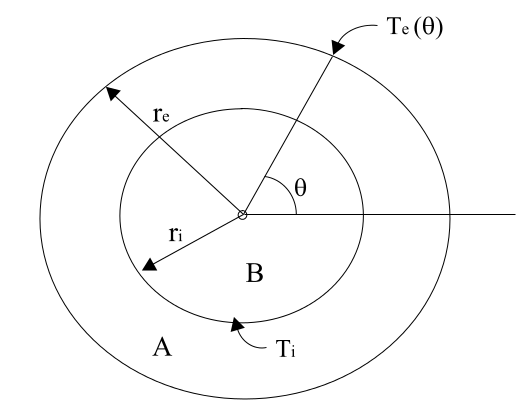
\includegraphics[width=0.6\columnwidth]{catedra/Horno.png}
\caption{Secci\'on circular del horno}
\end{center}
\end{figure}



El objetivo del trabajo práctico es implementar un programa que calcule la isoterma solicitada, conociendo las dimensiones del horno y las mediciones de temperatura en la pared exterior.

{\bf El Modelo}

Sea $r_e \in \mathbb{R}$ el radio exterior de la pared y sea $r_i \in \mathbb{R}$ el radio interior de la pared. Llamemos $T(r,\theta)$ a la temperatura en el punto dado por las coordenadas polares $(r,\theta)$, siendo $r$ el radio y $\theta$ el \'angulo polar de dicho punto. En el estado estacionario, esta temperatura satisface la ecuaci\'on del calor:

\begin{equation}\label{calor}
\frac{\partial^2T(r,\theta)}{\partial r^2}+\frac{1}{r}\frac{\partial T(r,\theta)}{\partial r}+\frac{1}{r^2}\frac{\partial^2T(r,\theta)}{\partial \theta^2} = 0 
\end{equation}


Si llamamos $T_i \in \mathbb{R}$ a la temperatura en el interior del horno (sector B) y $T_e : [0,2\pi] \rightarrow \mathbb{R}$ a la funci\'on de temperatura en el borde exterior del horno (de modo tal que el punto $(r_e,\theta)$ tiene temperatura $T_e(\theta)$), entonces tenemos que

\begin{equation}
T(r,\theta) = T_i \;\;\;\;\;para\;todo\;punto\;(r,\theta)\;con\;r\leq r_i
\end{equation}
\begin{equation}
T(r_e,\theta) = T_e(\theta) \;\;\;\;\;\;para\;todo\;punto\;(r_e,\theta)
\end{equation}


El problema en derivadas parciales dado por la primera ecuaci\'on con las condiciones de contorno presentadas recientemente, permite encontrar la funci\'on $T$ de temperatura en el interior del horno (sector A), en funci\'on de los datos mencionados en esta secci\'on.

Para resolver este problema computacionalmente, discretizamos el dominio del problema (el sector A) en coordenadas polares. Consideramos una partici\'on $0 = \theta_0 < \theta_1 < ... < \theta_n = 2\pi$ en $n$ \'angulos discretos con $\theta_k-\theta_{k-1} = \Delta\theta$ para $k = 1,...,n$, y una partici\'on $r_i = r_0 < r_1 < ... < r_m = r_e$ en $m+1$ radios discretos con $r_j - r_{j-1} = \Delta r$ para $j = 1,...,m$.

\medskip

El problema ahora consiste en determinar el valor de la funci\'on $T$ en los puntos de la discretizaci\'on $(r_j,\theta_k)$ que se encuentren dentro del sector A. Llamemos $t_{jk} = T(r_j,\theta_k)$ al valor (desconocido) de la funci\'on $T$ en el punto $(r_j,\theta_k)$.

\medskip

Para encontrar estos valores, transformamos la ecuaci\'on (\ref{calor}) en un conjunto de ecuaciones lineales sobre las inc\'ognitas $t_{jk}$, evaluando (\ref{calor}) en todos los puntos de la discretizaci\'on que se encuentren dentro del sector A. Al hacer esta evaluaci\'on, aproximamos las derivadas parciales de $T$ en (\ref{calor}) por medio de las siguientes f\'ormulas de diferencias finitas:


\begin{equation}
\frac{\partial^2T(r,\theta)}{\partial r^2}(r_j,\theta_k) \cong \frac{t_{j-1,k}-2t_{jk}+t_{j+1,k}}{(\Delta r)^2}
\end{equation}

\begin{equation}
\frac{\partial T(r,\theta)}{\partial r}(r_j,\theta_k) \cong \frac{t_{j,k}-t_{j-1,k}}{\Delta r}
\end{equation}

\begin{equation}
\frac{\partial^2T(r,\theta)}{\partial \theta^2}(r_j,\theta_k) \cong \frac{t_{j,k-1}-2t_{jk}+t_{j,k+1}}{(\Delta \theta)^2}
\end{equation}



Es importante notar que los valores de las inc\'ognitas son conocidos para los puntos que se encuentran sobre el borde exterior de la pared, y para los puntos que se encuentren dentro del sector B. Al realizar este procedimiento, obtenemos un sistema de ecuaciones lineales que modela el problema discretizado. La resoluci\'on de este sistema permite obtener una aproximaci\'on de los valores de la funci\'on $T$ en los puntos de la discretizaci\'on.

{\bf Enunciado}

Se debe implementar un programa en \verb+C+ o \verb-C++- que tome como entrada los par\'ametros del problema ($r_i$, $r_e$, $m+1$,
$n$, valor de la isoterma buscada, $T_i$, $T_e(\theta)$) que calcule la temperatura dentro de la pared del horno utilizando el
modelo propuesto en la secci\'on anterior y que encuentre la isoterma buscada en funci\'on del resultado obtenido del
sistema de ecuaciones. El m\'etodo para determinar la posici\'on de la isoterma queda a libre elecci\'on de cada grupo y
debe ser explicado en detalle en el informe.

El programa debe formular el sistema obtenido a partir de las ecuaciones (1) - (6) y considerar dos m\'etodos posibles
para su resoluci\'on: mediante el algoritmo cl\'asico de Eliminaci\'on Gaussiana y la Factorizaci\'on LU. Finalmente, el
programa escribir\'a en un archivo la soluci\'on obtenida con el formato especificado en la siguiente secci\'on.

Como ya se ha visto en la materia, no es posible aplicar los m\'etodos propuestos para la resoluci\'on a cualquier
sistema de ecuaciones. Sin embargo, la matriz del sistema considerado en el presente trabajo cumple con ser diagonal dominante (no
estricto) y que, ordenando las variables y ecuaciones convenientemente, es posible armar un sistema de ecuaciones cuya matriz
posee la propiedad de ser \emph{banda}. Luego, se pide demostrar (o al menos dar un esquema de la demostraci\'on)
el siguiente resultado e incluirlo en el informe:

\begin{proposition}
Sea $A \in \mathbb{R}^{n \times n}$ la matriz obtenida para el sistema definido por (1)-(6). Demostrar que es posible
aplicar Eliminaci\'on Gaussiana sin pivoteo.\footnote{Sugerencia: Notar que la matriz es diagonal dominante (no
estrictamente) y analizar qué sucede al aplicar un paso de Eliminaci\'on Gaussiana con los elementos de una fila.} 
\end{proposition}

La soluci\'on del sistema de ecuaciones permitir\'a saber la temperatura en los puntos de la discretizaci\'on. Sin embargo,
nuestro inter\'es es calcular la isoterma 500, para poder determinar si la estructura se encuentra en peligro. Luego, se pide lo siguiente:
\begin{itemize}
\item Dada la soluci\'on del sistema de ecuaciones, proponer una forma de estimar en cada \'angulo de la discretizaci\'on la posici\'on de la 
isoterma 500.
\item En funci\'on de la aproximaci\'on de la isoterma, proponer una forma (o medida) a utilizar para evaluar la peligrosidad de la estructura
en funci\'on de la distancia a la pared externa del horno.
\end{itemize}


En funci\'on de la experimentaci\'on, se busca realizar dos estudios complementarios: por un lado, analizar c\'omo se comporta el sistema y, por otro, 
cu\'ales son los requerimientos computacionales de los m\'etodos. Se pide como m\'inimo realizar los siguientes experimentos:
\begin{enumerate}
\item Comportamiento del sistema.
\begin{itemize}
\item Considerar al menos dos instancias de prueba, generando distintas discretizaciones para cada una de ellas y
comparando la ubicaci\'on de la isoterma buscada respecto de la pared externa del horno. Se sugiere presentar gr\'aficos
de temperatura o curvas de nivel para los mismos, ya sea utilizando las herramientas provistas por la c\'atedra o
implementando sus propias herramientas de graficaci\'on. 
\item Estudiar la proximidad de la isoterma buscada respecto de la pared exterior del horno en funci\'on de distintas 
granularidades de discretizaci\'on y las condiciones de borde. 
\end{itemize}
\item Evaluaci\'on de los m\'etodos.
\begin{itemize}
\item Analizar el tiempo de c\'omputo requerido para obtener la soluci\'on del sistema en funci\'on de la granularidad de 
la discretizaci\'on. Se sugiere presentar los resultados mediante gr\'aficos de tiempo de c\'omputo en funci\'on de alguna 
de las variables del problema.
\item Considerar un escenario similar al propuesto en el experimento 1. pero donde las condiciones de borde (i.e., $T_i$ y $T_e(\theta)$)
cambian en distintos instantes de tiempo. En este caso, buscamos obtener la secuencia de estados de la temperatura en
la pared del horno, y la respectiva ubicaci\'on de la isoterma especificada. Para ello, se considera una secuencia de $ninst$
vectores con las condiciones de borde, y las temperaturas en cada estado es la soluci\'on del correspondiente sistema de
ecuaciones. Se pide formular al menos un experimento de este tipo, aplicar los m\'etodos de resoluci\'on propuestos de
forma conveniente y compararlos en t\'erminos de tiempo total de c\'omputo requerido para distintos valores de $ninst$.
\end{itemize}
\end{enumerate}

De manera opcional, aquellos grupos que quieran ir un poco m\'as all\'a pueden considerar trabajar y desarrollar alguno(s) 
de los siguientes puntos extra:
\begin{enumerate}
\item Notar que el sistema resultante tiene estructura \emph{banda}. Proponer una estructura para aprovechar este hecho en t\'erminos de la
\emph{complejidad espacial} y como se adaptar\'ian los algoritmos de Eliminaci\'on Gaussiana y Factorizaci\'on LU para reducir la
cantidad de operaciones a realizar.
\item Implementar dicha estructura y las adaptaciones necesarias para el algoritmo de Eliminaci\'on Gaussiana.
\item Implementar dicha estructura y las adaptaciones necesarias para el algoritmo de Factorizaci\'on LU. 
\end{enumerate}

Finalmente, se deber\'a presentar un informe que incluya una descripci\'on detallada de los m\'etodos implementados y
las decisiones tomadas, el m\'etodo propuesto para el c\'alculo de la isoterma buscada y los experimentos realizados,
junto con el correspondiente an\'alisis y siguiendo las pautas definidas en el archivo \verb+pautas.pdf+.

{\bf Programa y formato de archivos}

Se deber\'an entregar los archivos fuentes que contengan la resoluci\'on del trabajo pr\'actico. El ejecutable tomar\'a
tres par\'ametros por l\'inea de comando, que ser\'an el archivo de entrada, el archivo de salida, y el m\'etodo a
ejectutar (0 EG, 1 LU).

El archivo de entrada tendr\'a la siguiente estructura:
\begin{itemize}
\item La primera l\'inea contendr\'a los valores $r_i$, $r_e$, $m+1$, $n$, $iso$, $ninst$, donde $iso$ representa el
valor de la isoterma buscada y $ninst$ es la cantidad de instancias del problema a resolver para los par\'ametros dados.
\item A continuaci\'on, el archivo contendr\'a $ninst$ l\'ineas, cada una de ellas con $2n$ valores, los primeros $n$ indicando los
valores de la temperatura en la pared interna, i.e., $T_i(\theta_0),T_i(\theta_1),\dots,T_i(\theta_{n-1})$, seguidos de $n$ valores
de la temperatura en la pared externa, i.e., $T_e(\theta_0)$,$T_e(\theta_1)$,$\dots$,$T_e(\theta_{n-1})$.
\end{itemize}

El archivo de salida obligatorio tendr\'a el vector soluci\'on del sistema reportando una componente del mismo por
l\'inea. En caso de $ninst > 1$, los vectores ser\'an reportados uno debajo del otro.

Junto con el presente enunciado, se adjunta una serie de scripts hechos en \verb+python+ y un conjunto instancias de
test que deber\'an ser utilizados para la compilaci\'on y un testeo b\'asico de la implementaci\'on. Se recomienda leer
el archivo \verb+README.txt+ con el detalle sobre su utilizaci\'on.

{\bf \underline{Fechas de entrega}}
\begin{itemize}
\item \emph{Formato Electr\'onico:} Jueves 3 de Septiembre de 2015, hasta las 23:59 hs, enviando el trabajo (informe +
c\'odigo) a la direcci\'on \verb+metnum.lab@gmail.com+. El subject del email debe comenzar con el texto \verb+[TP1]+
seguido de la lista de apellidos de los integrantes del grupo.
\item \emph{Formato f\'isico:} Viernes 4 de Septiembre de 2015, de 17:30 a 18:00 hs.
\end{itemize}

\noindent \textbf{Importante:} El horario es estricto. Los correos recibidos despu\'es de la hora indicada ser\'an
considerados re-entrega. Los grupos deben ser de 3 o 4 personas, sin excepci\'on. Es indispensable que los trabajos
pasen satisfactoriamente los casos de test provistos por la c\'atedra.
\section{Apéndice B: Código}
\subsection{matrix.h}
\lstinputlisting[language=C++, breaklines=true]{../src/src/matrix.h}
\subsection{eqsys.h}
\lstinputlisting[language=C++, breaklines=true]{../src/src/eqsys.h}
\subsection{buildSystem.cpp}
\lstinputlisting[language=C++, breaklines=true]{../src/src/buildSystem.cpp}

\end{document}